\documentclass[tikz, preview]{standalone}

\usepackage{amsfonts, amsthm, amssymb, amsmath, stmaryrd, etoolbox}
\usepackage{tikz}
\usepackage[all,2cell]{xy}
\usetikzlibrary{matrix,arrows,shapes,decorations.markings,decorations.pathreplacing}
\definecolor{rewritecolor}{rgb}{0,.9,1}
\tikzset{rewritenode/.style={shape=circle,fill=rewritecolor,scale=0.25,font=\Huge}}
\tikzset{RWopen/.style={shape=circle,draw=black,fill=white,scale=0.5,font=\Huge}}
\tikzset{RWclosed/.style={shape=circle,fill=black,scale=0.5,font=\Huge}}
\tikzset{CDnode/.style={shape=circle,fill=white,scale=.5}}
\tikzset{zxgreen/.style={shape=circle,draw,thick,fill=green}}
\tikzset{zxred/.style={shape=circle,draw,thick,fill=red}}
\tikzset{zxyellow/.style={shape=rectangle,draw,thick,fill=yellow}}
\tikzset{zxdiamond/.style={shape=diamond,fill=black,inner sep=2.75}}
\tikzset{zxopen/.style={shape=circle,draw,thick,inner sep=2pt}}
\tikzset{->-/.style={decoration={markings,mark=at position .5 with {\arrow{>}}},postaction={decorate}}}

\begin{document}
\[
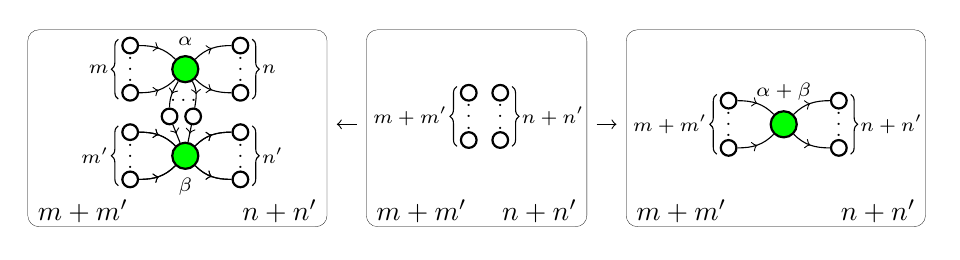
\begin{tikzpicture}
\begin{scope}[shift={(-1.2,0.1)}]
\node [zxgreen,label={\scriptsize $\alpha$}] (v1) at (-0.9,0.1) {};
\node [zxopen] (v2) at (-1.6,0.4) {};
\node [zxopen] (v3) at (-1.6,-0.2) {};
\node [zxopen] (v4) at (-0.2,0.4) {};
\node [zxopen] (v5) at (-0.2,-0.2) {};
\node [zxgreen,label={[shift={(0,-0.8)}]\scriptsize $\beta$}] (v6) at (-0.9,-1) {};
\node [zxopen] (v7) at (-1.6,-0.7) {};
\node [zxopen] (v8) at (-1.6,-1.3) {};
\node [zxopen] (v9) at (-0.2,-0.7) {};
\node [zxopen] (v10) at (-0.2,-1.3) {};
\node [zxopen] (v11) at (-1.1,-0.5) {};
\node [zxopen] (v12) at (-0.8,-0.5) {};
%
\draw [->-] (v2) to [in=135,out=0] (v1);
\draw [->-] (v3) to [in=-135,out=0] (v1);
\draw [->-] (v1) to [in=180,out=45] (v4);
\draw [->-] (v1) to [in=180,out=-45] (v5);
\draw [->-] (v7) to [in=135,out=0] (v6);
\draw [->-] (v8) to [in=-135,out=0] (v6);
\draw [->-] (v6) to [in=180,out=45] (v9);
\draw [->-] (v6) to [in=180,out=-45] (v10);
\draw [->-] (v1) to [out=-60,in=80] (v12);
\draw [->-] (v12) to [bend left=0] (v6);
\draw [->-] (v1) to [out=-120,in=90] (v11);
\draw [->-] (v11) to [bend right=0] (v6);
\node at (-1.6,0.2) {\scriptsize $\vdots$};
\node at (-0.2,0.2) {\scriptsize $\vdots$};
\node at (-1.6,-0.9) {\scriptsize $\vdots$};
\node at (-0.2,-0.9) {\scriptsize $\vdots$};
\node at (-0.9,-0.3) {\scriptsize $\dots$};
%
\draw[decoration={brace,mirror,raise=2pt},decorate]
(v2.north west) -- node [left=2pt] {\scriptsize $m$} (v3.south west); 
\draw[decoration={brace,mirror,raise=2pt},decorate]
(v7.north west) -- node [left=2pt] {\scriptsize $m'$} (v8.south west);
\draw[decoration={brace,raise=2pt},decorate]
(v4.north east) -- node [right=2pt] {\scriptsize $n$} (v5.south east); 
\draw[decoration={brace,raise=2pt},decorate]
(v9.north east) -- node [right=2pt] {\scriptsize $n'$} (v10.south east); 
%
\node at (-2.2,-1.7) {$m+m'$};
\node at (0.3,-1.7) {$n+n'$};
\node (a1) at (0.9,-0.6) {};
\draw [ultra thin, rounded corners] (-2.9,0.6) rectangle (0.9,-1.9);
\end{scope}
%
%
%
\begin{scope}[shift={(3.2,-0.1)}]
\node [zxopen] (v1) at (-1.7,0) {};
\node [zxopen] (v2) at (-1.3,0) {};
\node [zxopen] (v3) at (-1.7,-0.6) {};
\node [zxopen] (v4) at (-1.3,-0.6) {};
\node at (-1.7,-0.2) {\scriptsize $\vdots$};
\node at (-1.3,-0.2) {\scriptsize $\vdots$};
%
\draw [ultra thin, rounded corners] (-3,0.8) rectangle (-0.2,-1.7);
\draw[decoration={brace,mirror,raise=2pt},decorate]
(v1.north west) -- node [left=2pt] {\scriptsize $m+m'$} (v3.south west);
\draw[decoration={brace,raise=2pt},decorate]
(v2.north east) -- node [right=2pt] {\scriptsize $n+n'$} (v4.south east); 
\node at (-2.3,-1.5) {$m+m'$};
\node at (-0.8,-1.5) {$n+n'$};
\node (a2) at (-3,-0.4) {};
\node (a3) at (-0.2,-0.4) {};
\end{scope}
%
%
%
\begin{scope}[shift={(5.5,-0.5)}]
\node [zxgreen,label={\scriptsize $\alpha+\beta$}] (v1) at (0,0) {};
\node [zxopen] (v2) at (-0.7,0.3) {};
\node [zxopen] (v3) at (-0.7,-0.3) {};
\node [zxopen] (v4) at (0.7,0.3) {};
\node [zxopen] (v5) at (0.7,-0.3) {};
%
\draw [->-] (v2) to [in=135,out=0] (v1);
\draw [->-] (v3) to [in=-135,out=0] (v1);
\draw [->-] (v1) to [in=180,out=45] (v4);
\draw [->-] (v1) to [in=180,out=-45] (v5);
\draw [->-] (v7) to [in=135,out=0] (v6);
\draw [->-] (v8) to [in=-135,out=0] (v6);
\draw [->-] (v6) to [in=180,out=45] (v9);
\draw [->-] (v6) to [in=180,out=-45] (v10);
\node at (-0.7,0.1) {\scriptsize $\vdots$};
\node at (0.7,0.1) {\scriptsize $\vdots$};
%
\draw[decoration={brace,mirror,raise=2pt},decorate]
(v2.north west) -- node [left=2pt] {\scriptsize $m+m'$} (v3.south west); 
\draw[decoration={brace,raise=2pt},decorate]
(v4.north east) -- node [right=2pt] {\scriptsize $n+n'$} (v5.south east); 
%
\node at (-1.3,-1.1) {$m+m'$};
\node at (1.2,-1.1) {$n+n'$};
\draw [ultra thin, rounded corners] (-2,1.2) rectangle (1.8,-1.3);
\node (a4) at (-2,0) {};
\end{scope}
%
%
%
\draw [<-] (a1) edge (a2);
\draw [->] (a3) edge (a4);
\end{tikzpicture}
\]
\end{document}
